% Chapter 1

\chapter{TDSE Solutions for Time-Dependent Potentials} % Main chapter title

\label{Chapter4} % For referencing the chapter elsewhere, use \ref{Chapter1} 

%----------------------------------------------------------------------------------------
\section{Qualitative Expectation for Results}
Previously we saw that solutions to the TISE can be expressed as weighted sums of bound eigenstates, where each bound eigenstate corresponds to a distinct energy. It was also shown that if no external potential acts on the system these weights will not change as the wavefunction evolves with time; we used this fact to measure the accuracy of our propagators in the previous chapter. 

The fact that these weights remain constant with no external potential being applied is equivalent to saying that the energy of the system remains constant under time evolution; this makes physical sense as a statement of the conservation of energy. When an external field is applied, the system will either gain or lose energy over time - and so these weights will change during time evolution. 

As the weight / coefficient of each eigenstate corresponds to the probability of the system being in that state, by constructing appropriate time-dependent external potentials we can model how the probabilities of the system being in particular eigenstates changes in the event of some physical interactions; for example absorbing a laser pulse. 

The rest of this chapter consists of investigating how the system, initially in the Ground State, evolves under the influence of different simulated interactions - by investigating the change to the Ground State population under the interactions over time.

\section{DC Drift}
Here we investigate the evolution of the system under a linearly growing (w.r.t. time) potential field; similar to a voltage applied from a DC power source.

\subsection{Potential Description}
We simulate the external potential term as $\alpha t \mathbf{r}$; where $\mathbf{r}$ is the spatial interval, $t$ is the time, and $\alpha$ is a constant to determine the intensity of the DC potential.

This extra potential term was then added to the softcore potential, and the resulting total potential used along the central diagonal of the Hamiltonian.

\subsection{Effect On State Evolution}
Figure 4.1, below, shows the effect of the DC potential on the wavefunction (initially Ground State) over time.
\begin{figure}[H]
          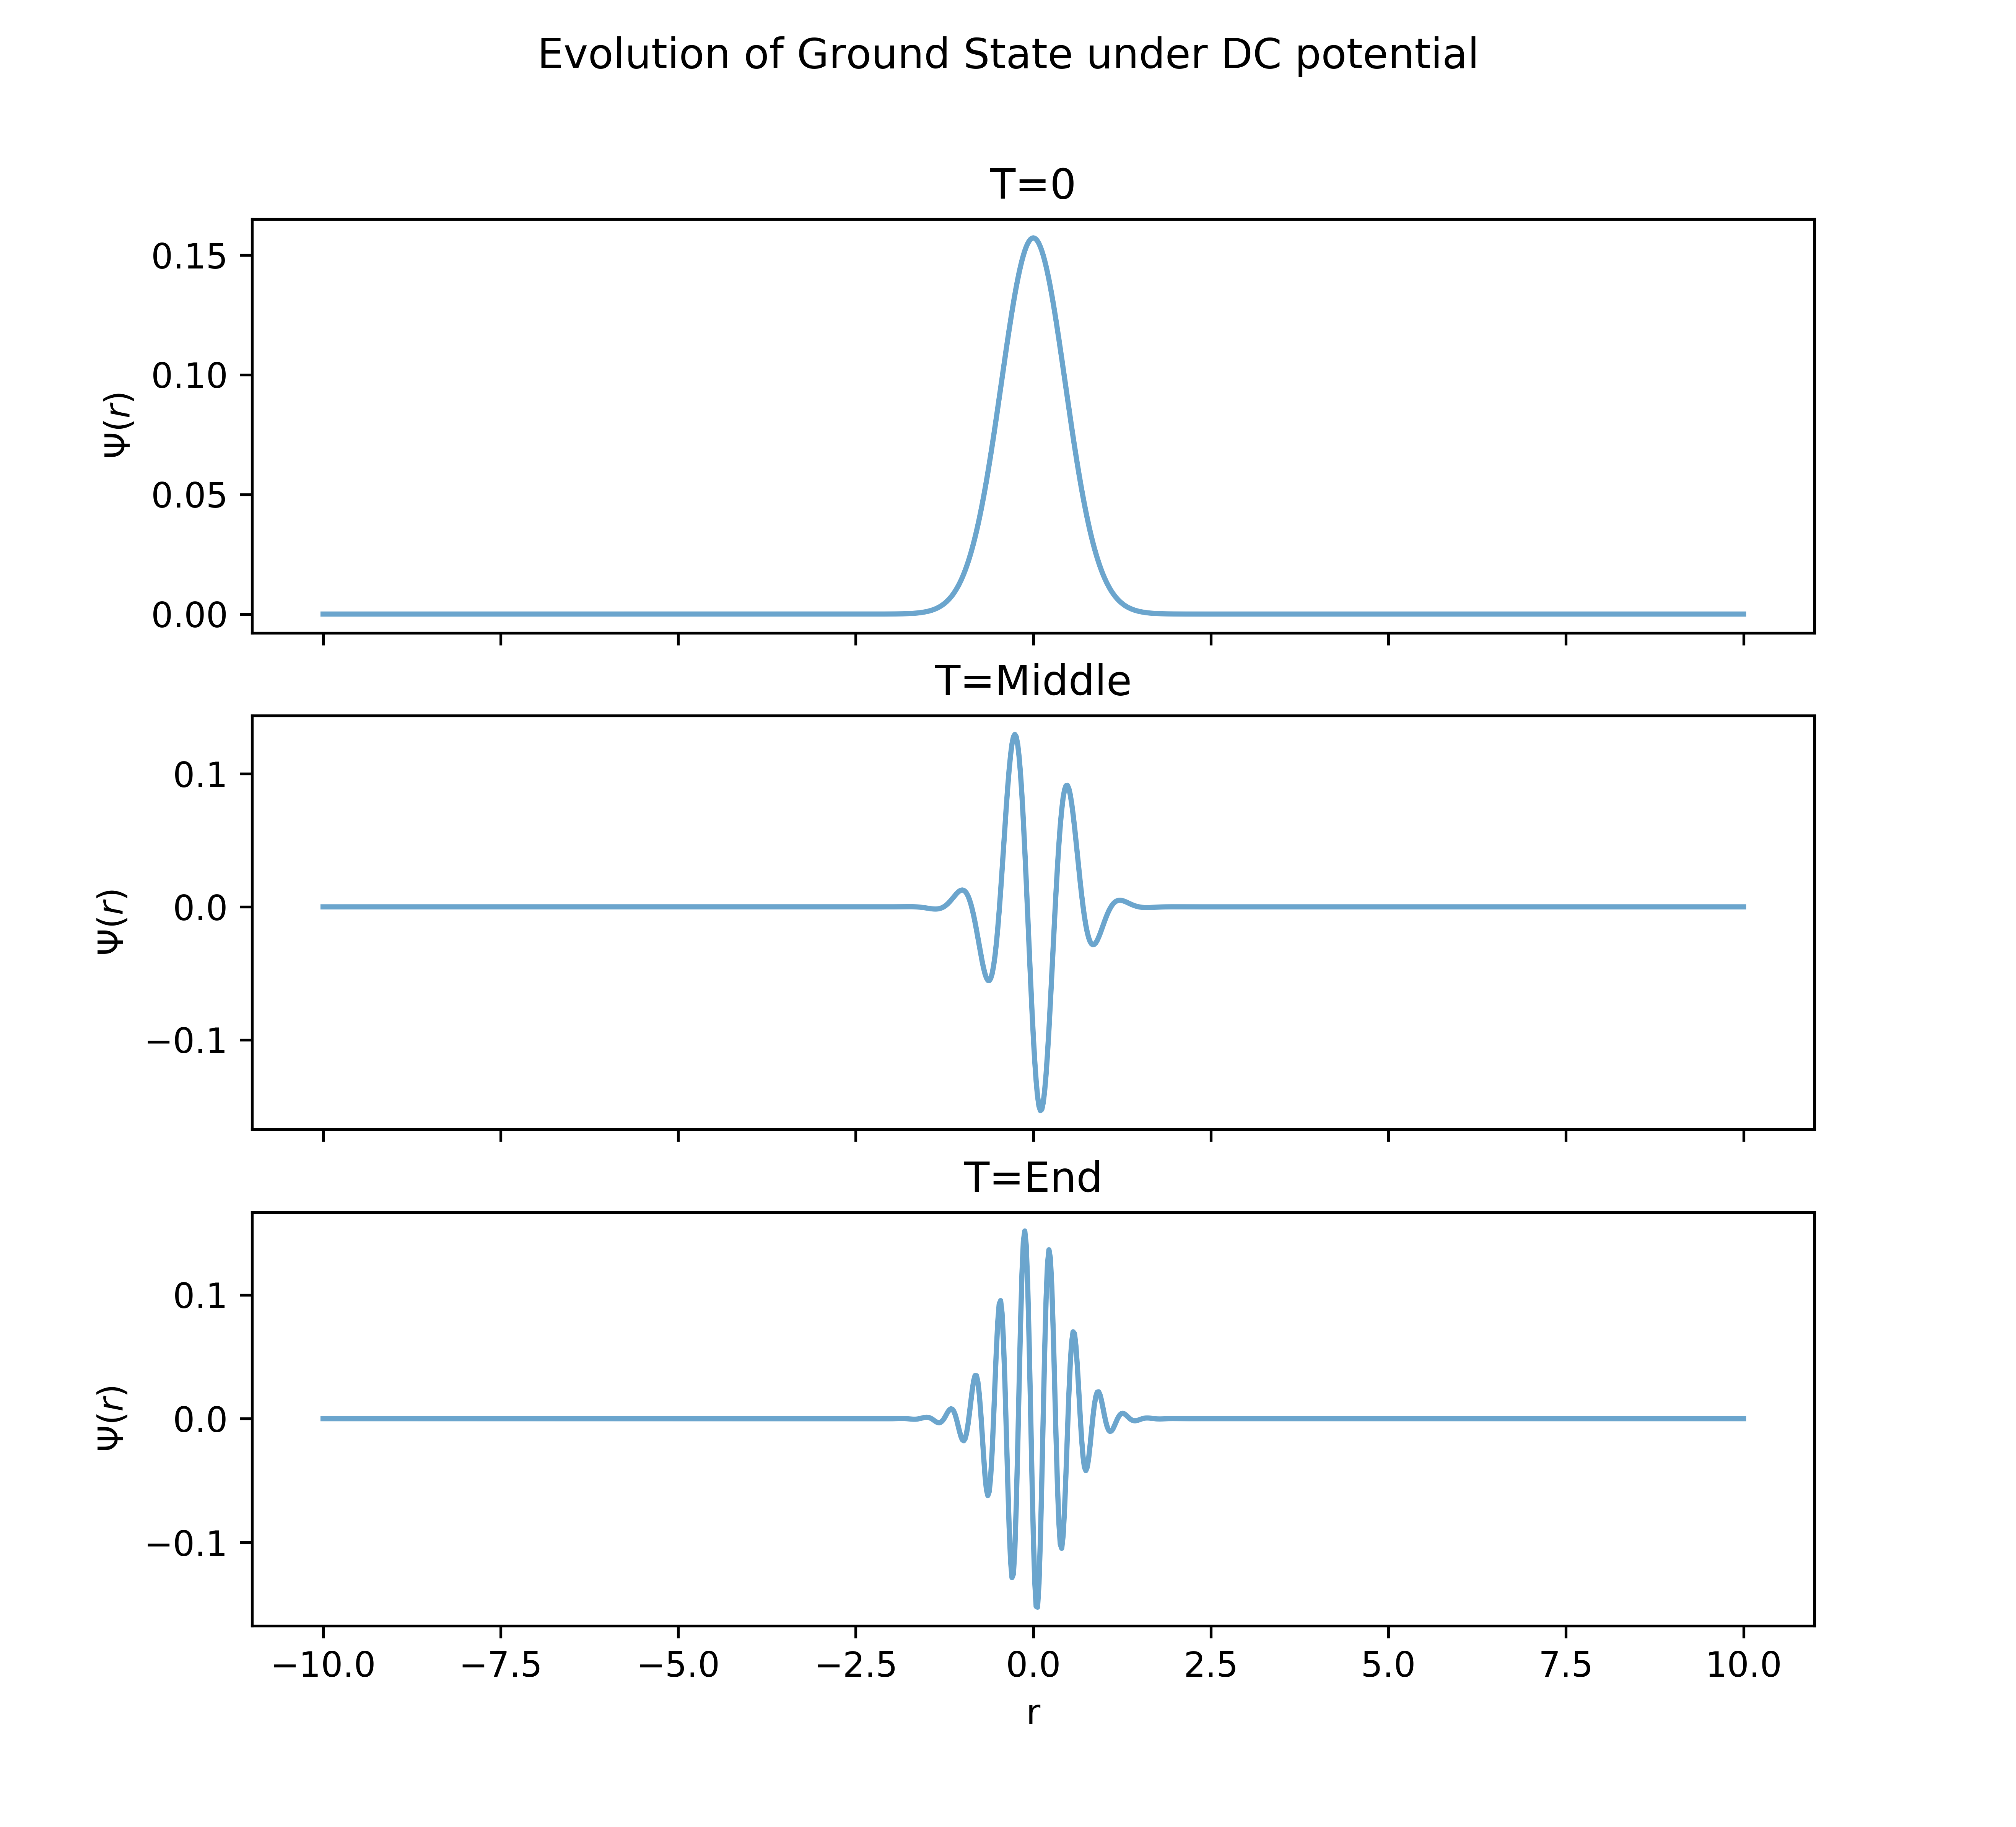
\includegraphics[width=\textwidth]{./GSDCwavefunction3times.png}
          \centering
          \caption{Effect of DC potential on wavefunction}
\end{figure}
From this figure, we see qualitatively that as time goes on the system is excited to higher and higher energies; shown through the increased numbers of turning points, and their relative magnitudes, indicating increasing contributions from higher energy eigenstates. Based on this, we can expect that the Ground State population will reduce over time as more and more eigenstates contribute and their contributions gain more and more weight. Figure 4.2, below, shows the decrease in the Ground State population over the same time interval:

\begin{figure}[H]
          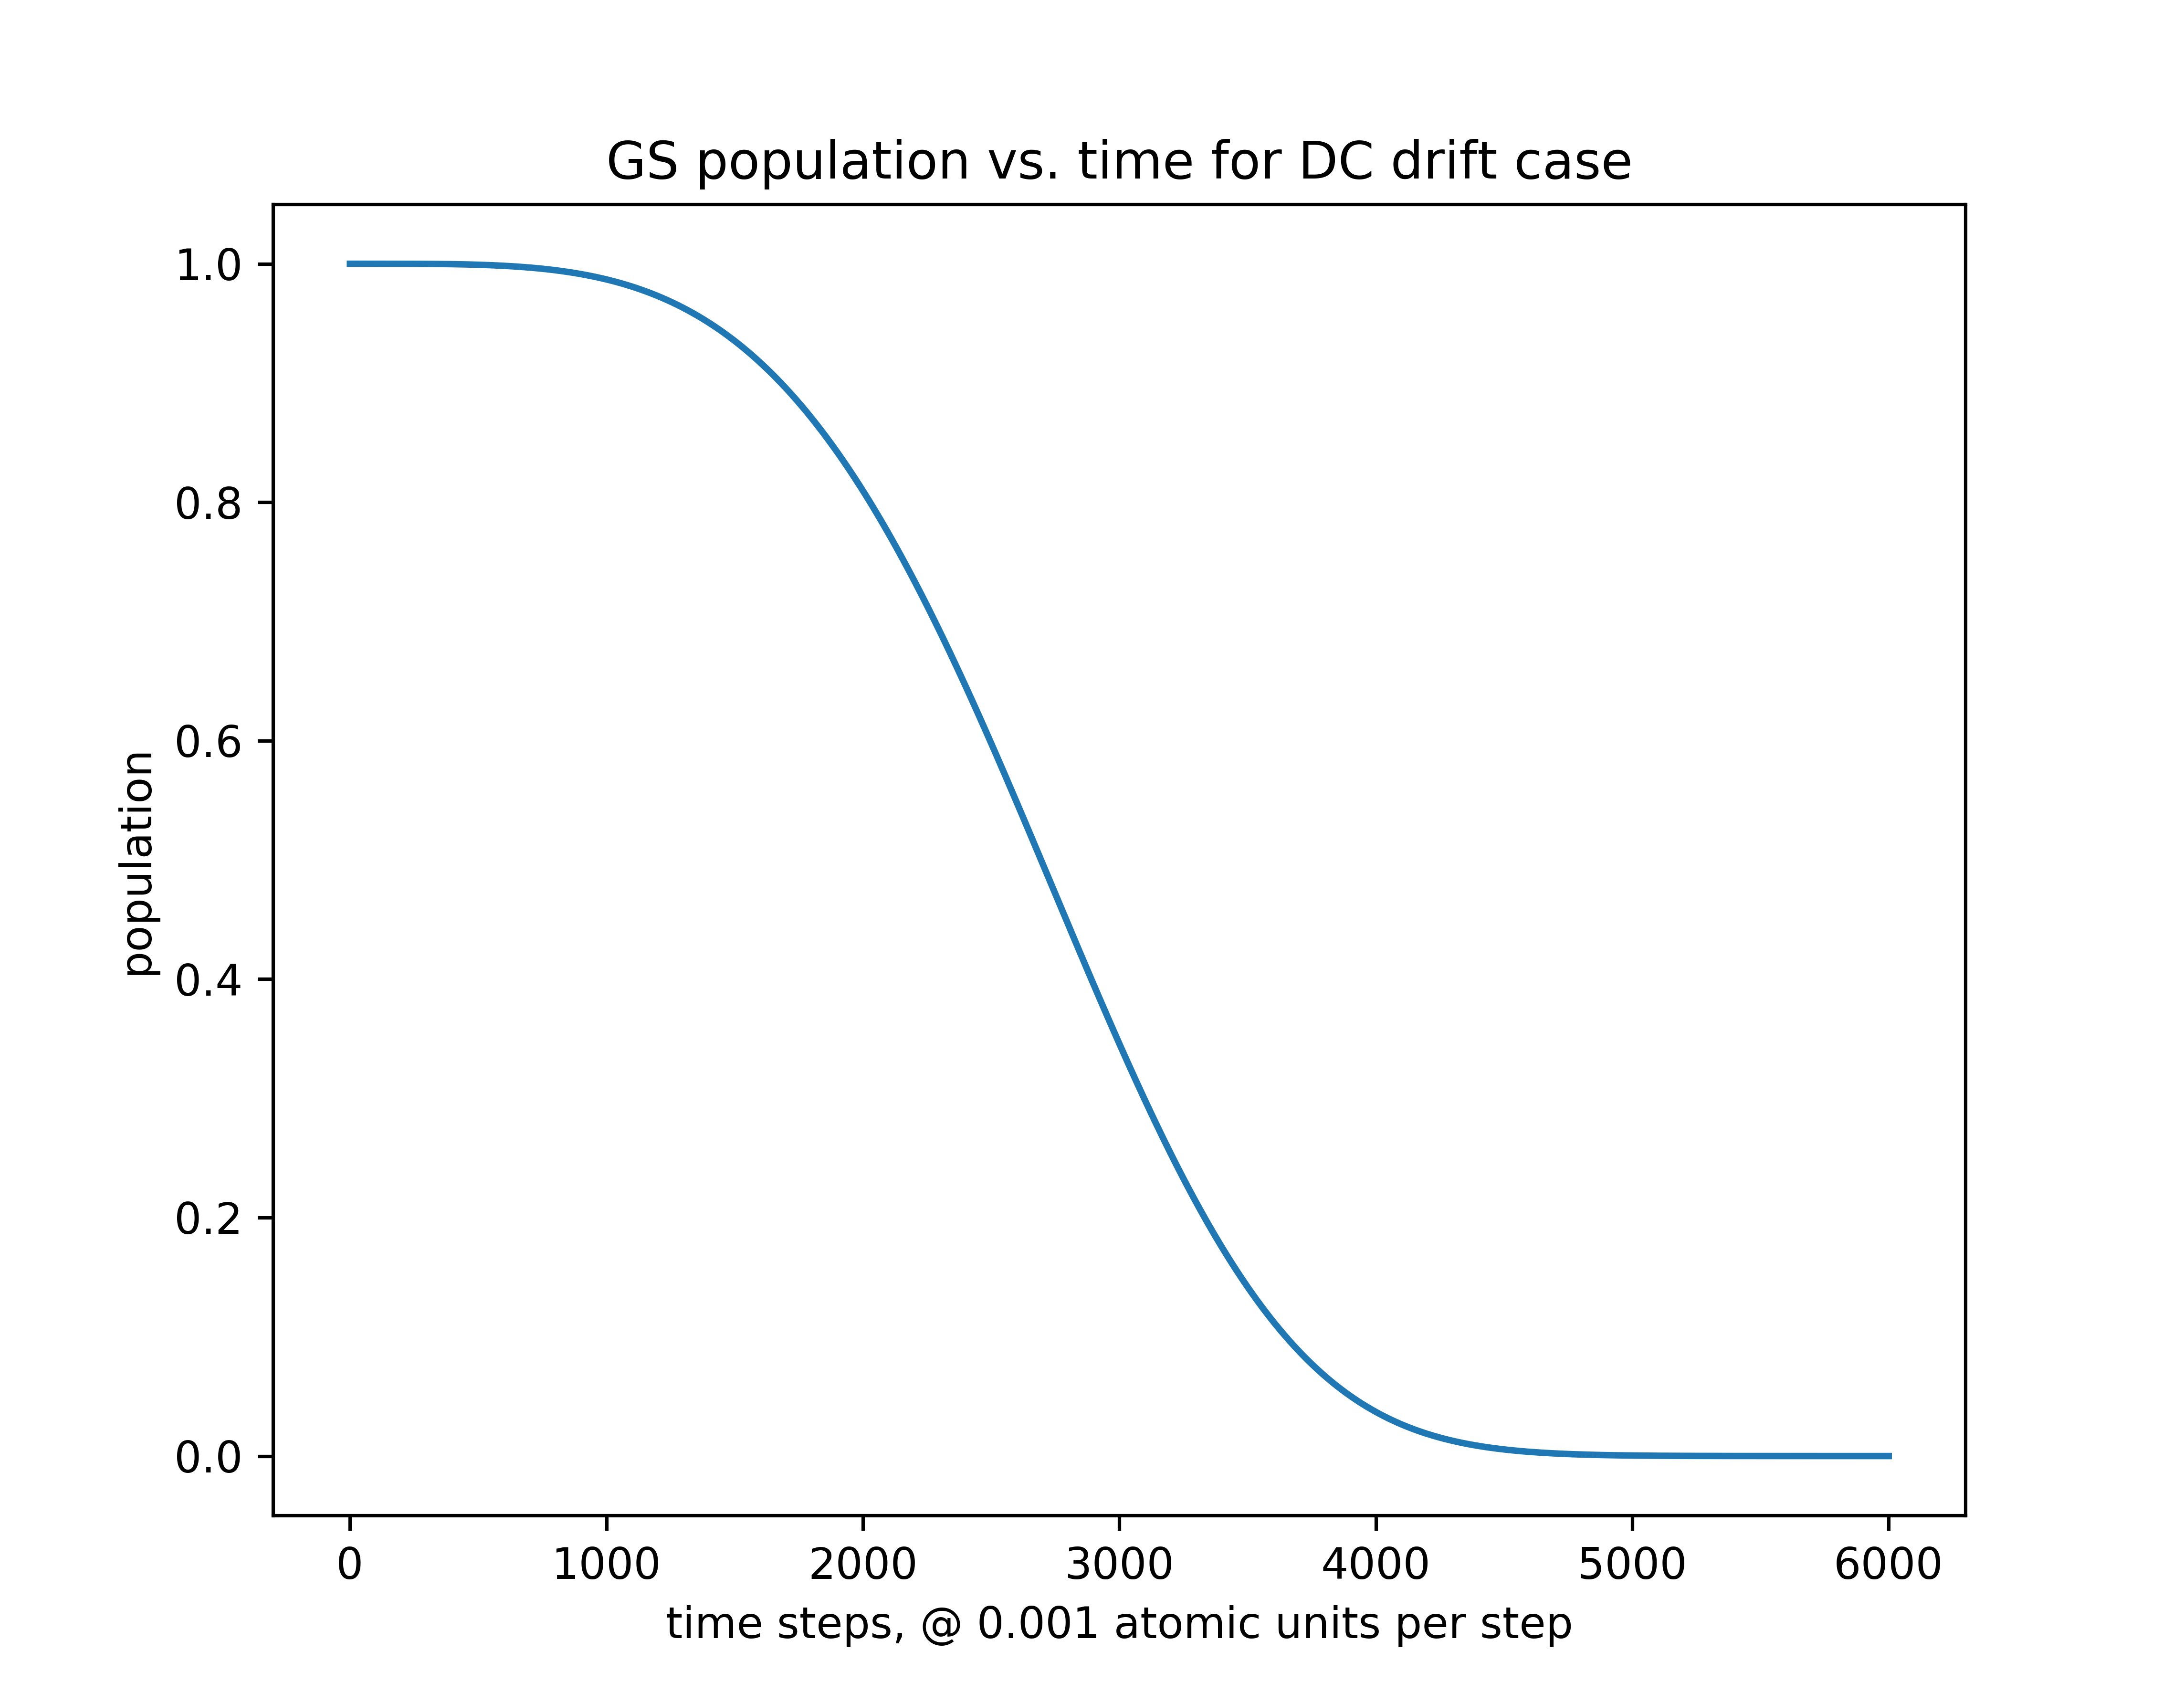
\includegraphics[width=\textwidth]{./GSpopDC.png}
          \centering
          \caption{Effect of DC potential on Ground State Population}
\end{figure}

\section{Simulated `Laser Pulse' Potential}
In this section we investigate how our system would behave under the influence of a laser pulse.

\subsection{Potential Description}
In this case, we simulate the external potential term as a gaussian packet w.r.t. time such that the centre of the packet (most intense part) occurs at 1 atomic unit of time, and the standard deviation of the packet is 0.25 atomic units of time. The intensity of the laser pulse is controlled by a multiplicative factor, $\alpha$, giving the following expression for the external potential: 
$$
V_{\text{ext}} = \alpha \frac{4}{\sqrt{2\pi}}e^{-8\left(t-1\right)^{2}}\mathbf{r}
$$

As with the previous example, this extra potential term was added to the softcore potential, and the result used along the central diagonal of the Hamiltonian.

\subsection{Effect On State Evolution}

\begin{figure}[H]
          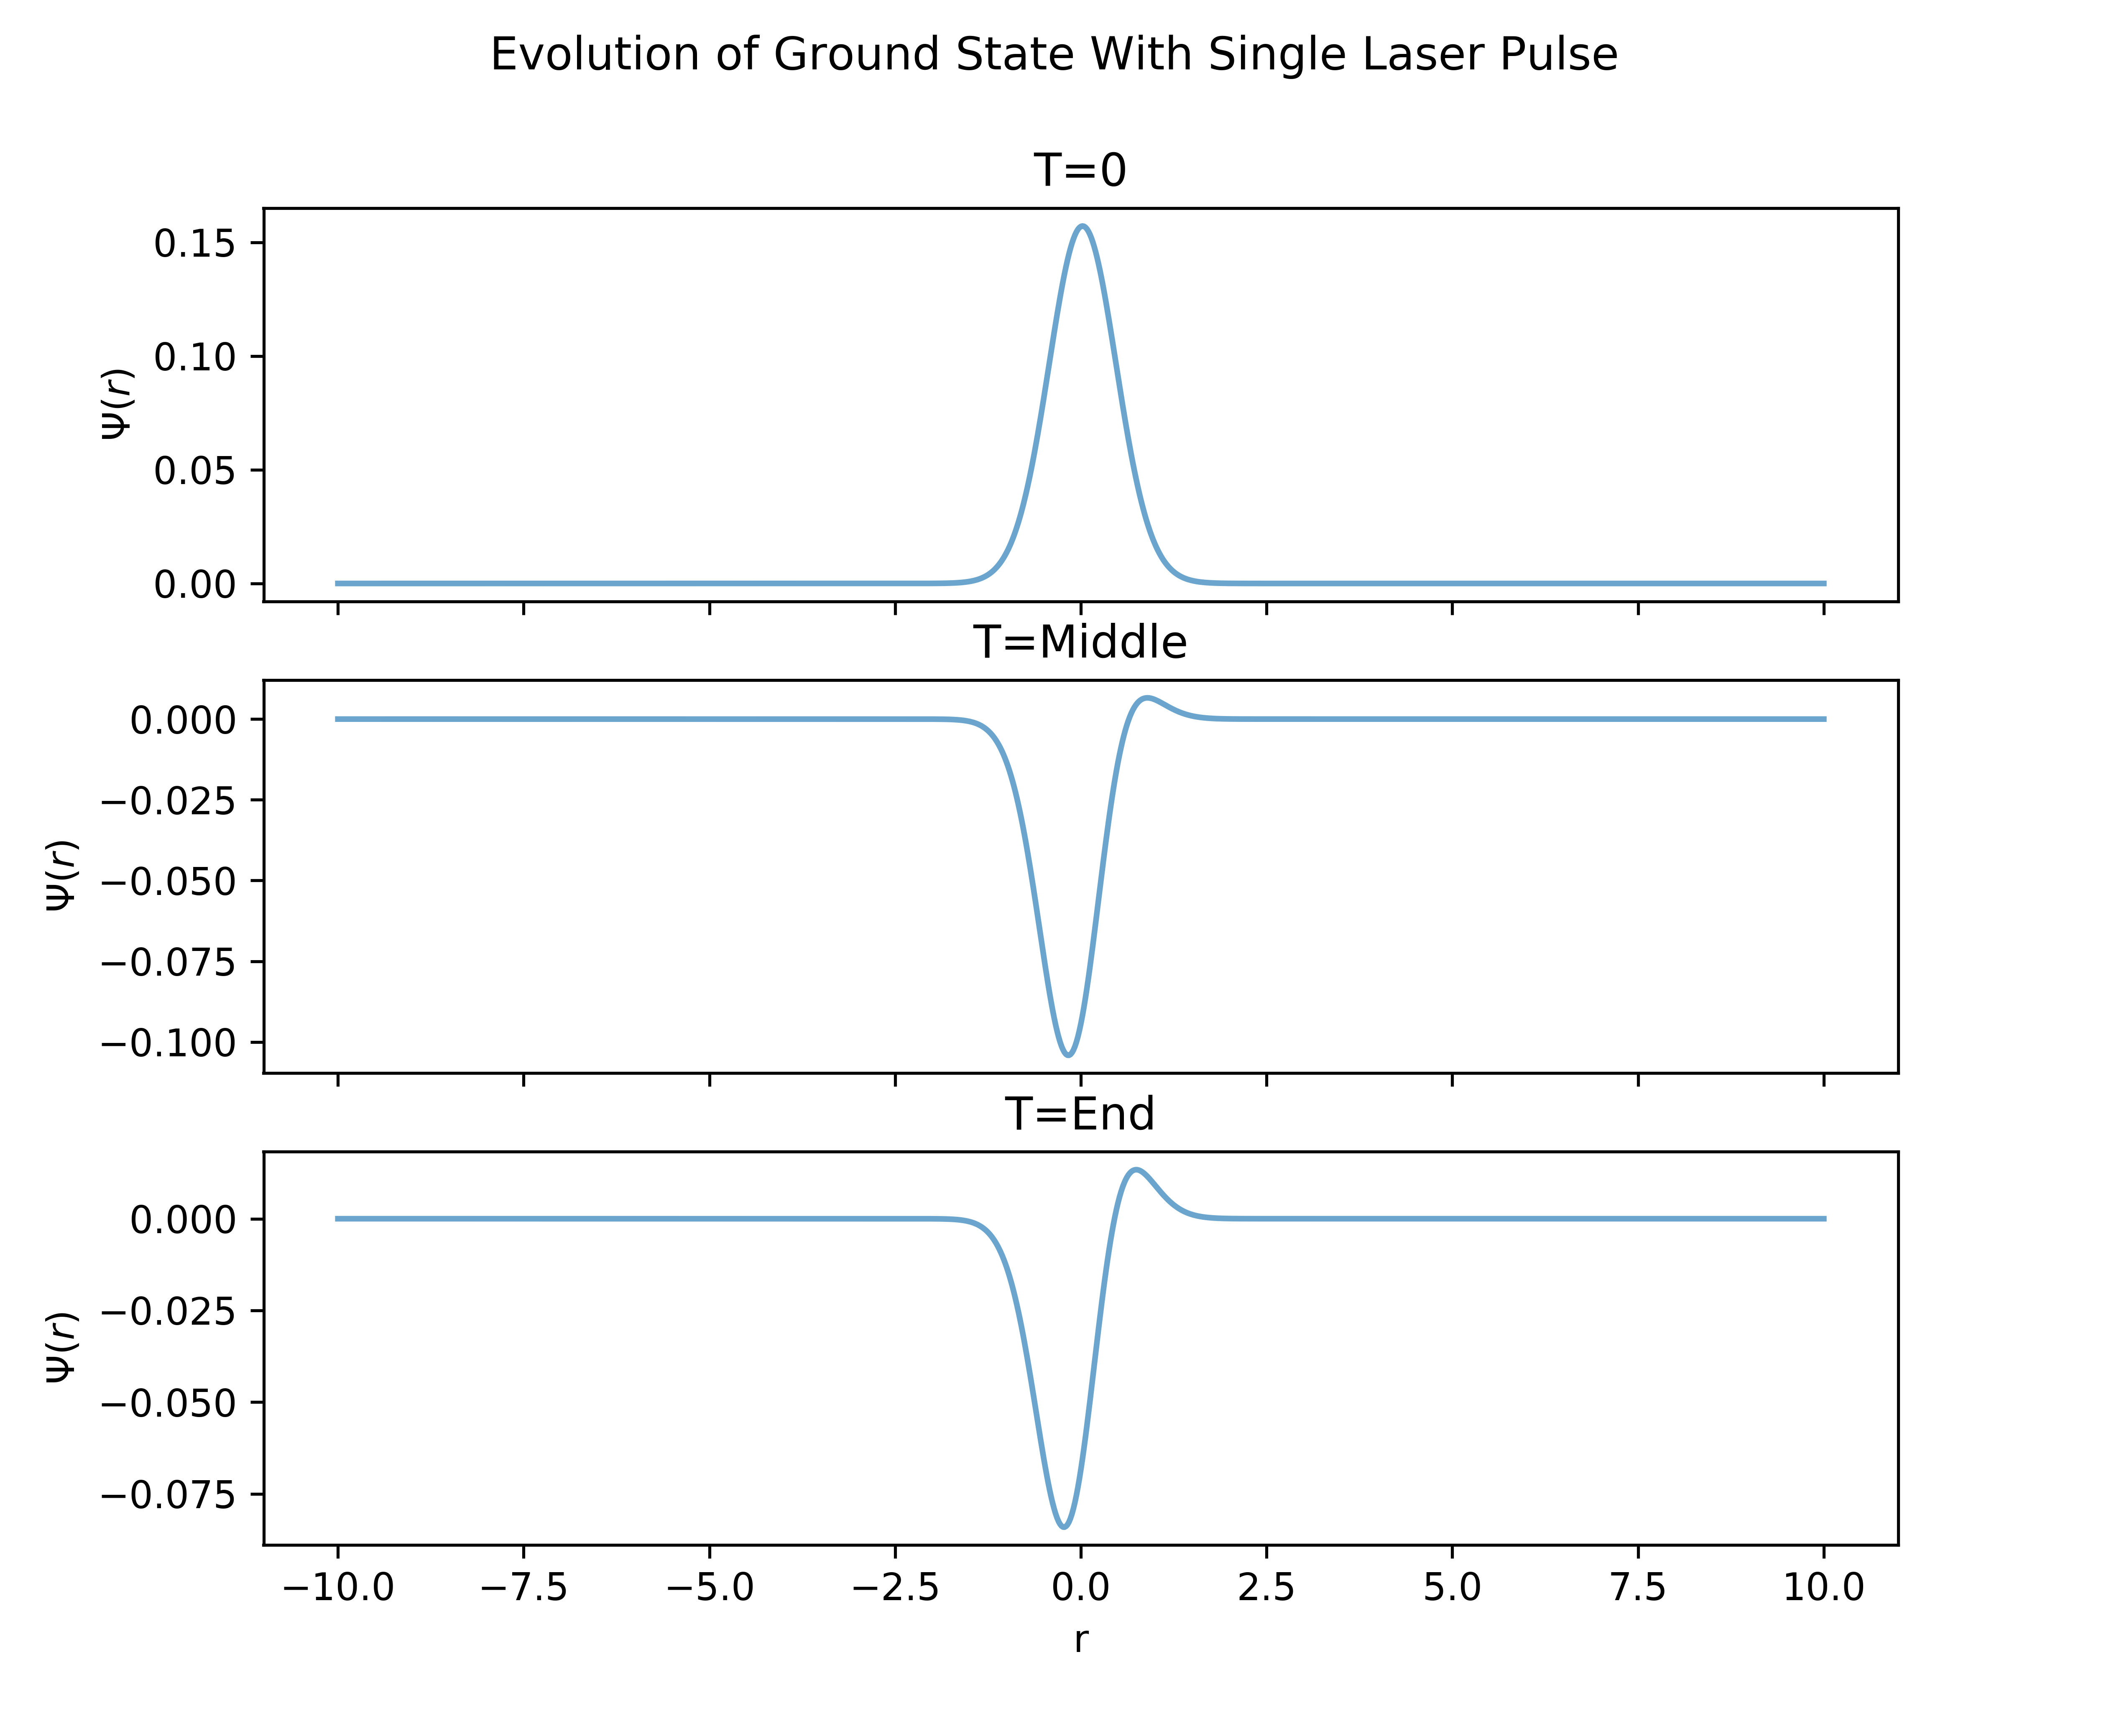
\includegraphics[width=\textwidth]{./GS1LPwavefunction3times.png}
          \centering
          \caption{Effect of Single Laser Pulse on wavefunction}
\end{figure}

Figure 4.3, above, we see that almost all of a relatively small amount of energy is absorbed some time between the start and mid-point of the simulation (an interval of 3 atomic units of time), seen through the small additional turning point indicating a small contribution from the first excited state. There is very little change in shape between the mid-point and end of the simulation, indicating that there was very little incoming / outgoing energy in this time period.

The change to Ground State population was investigated over the same time interval, and the results shown in Figure 4.4, below:
\begin{figure}[H]
          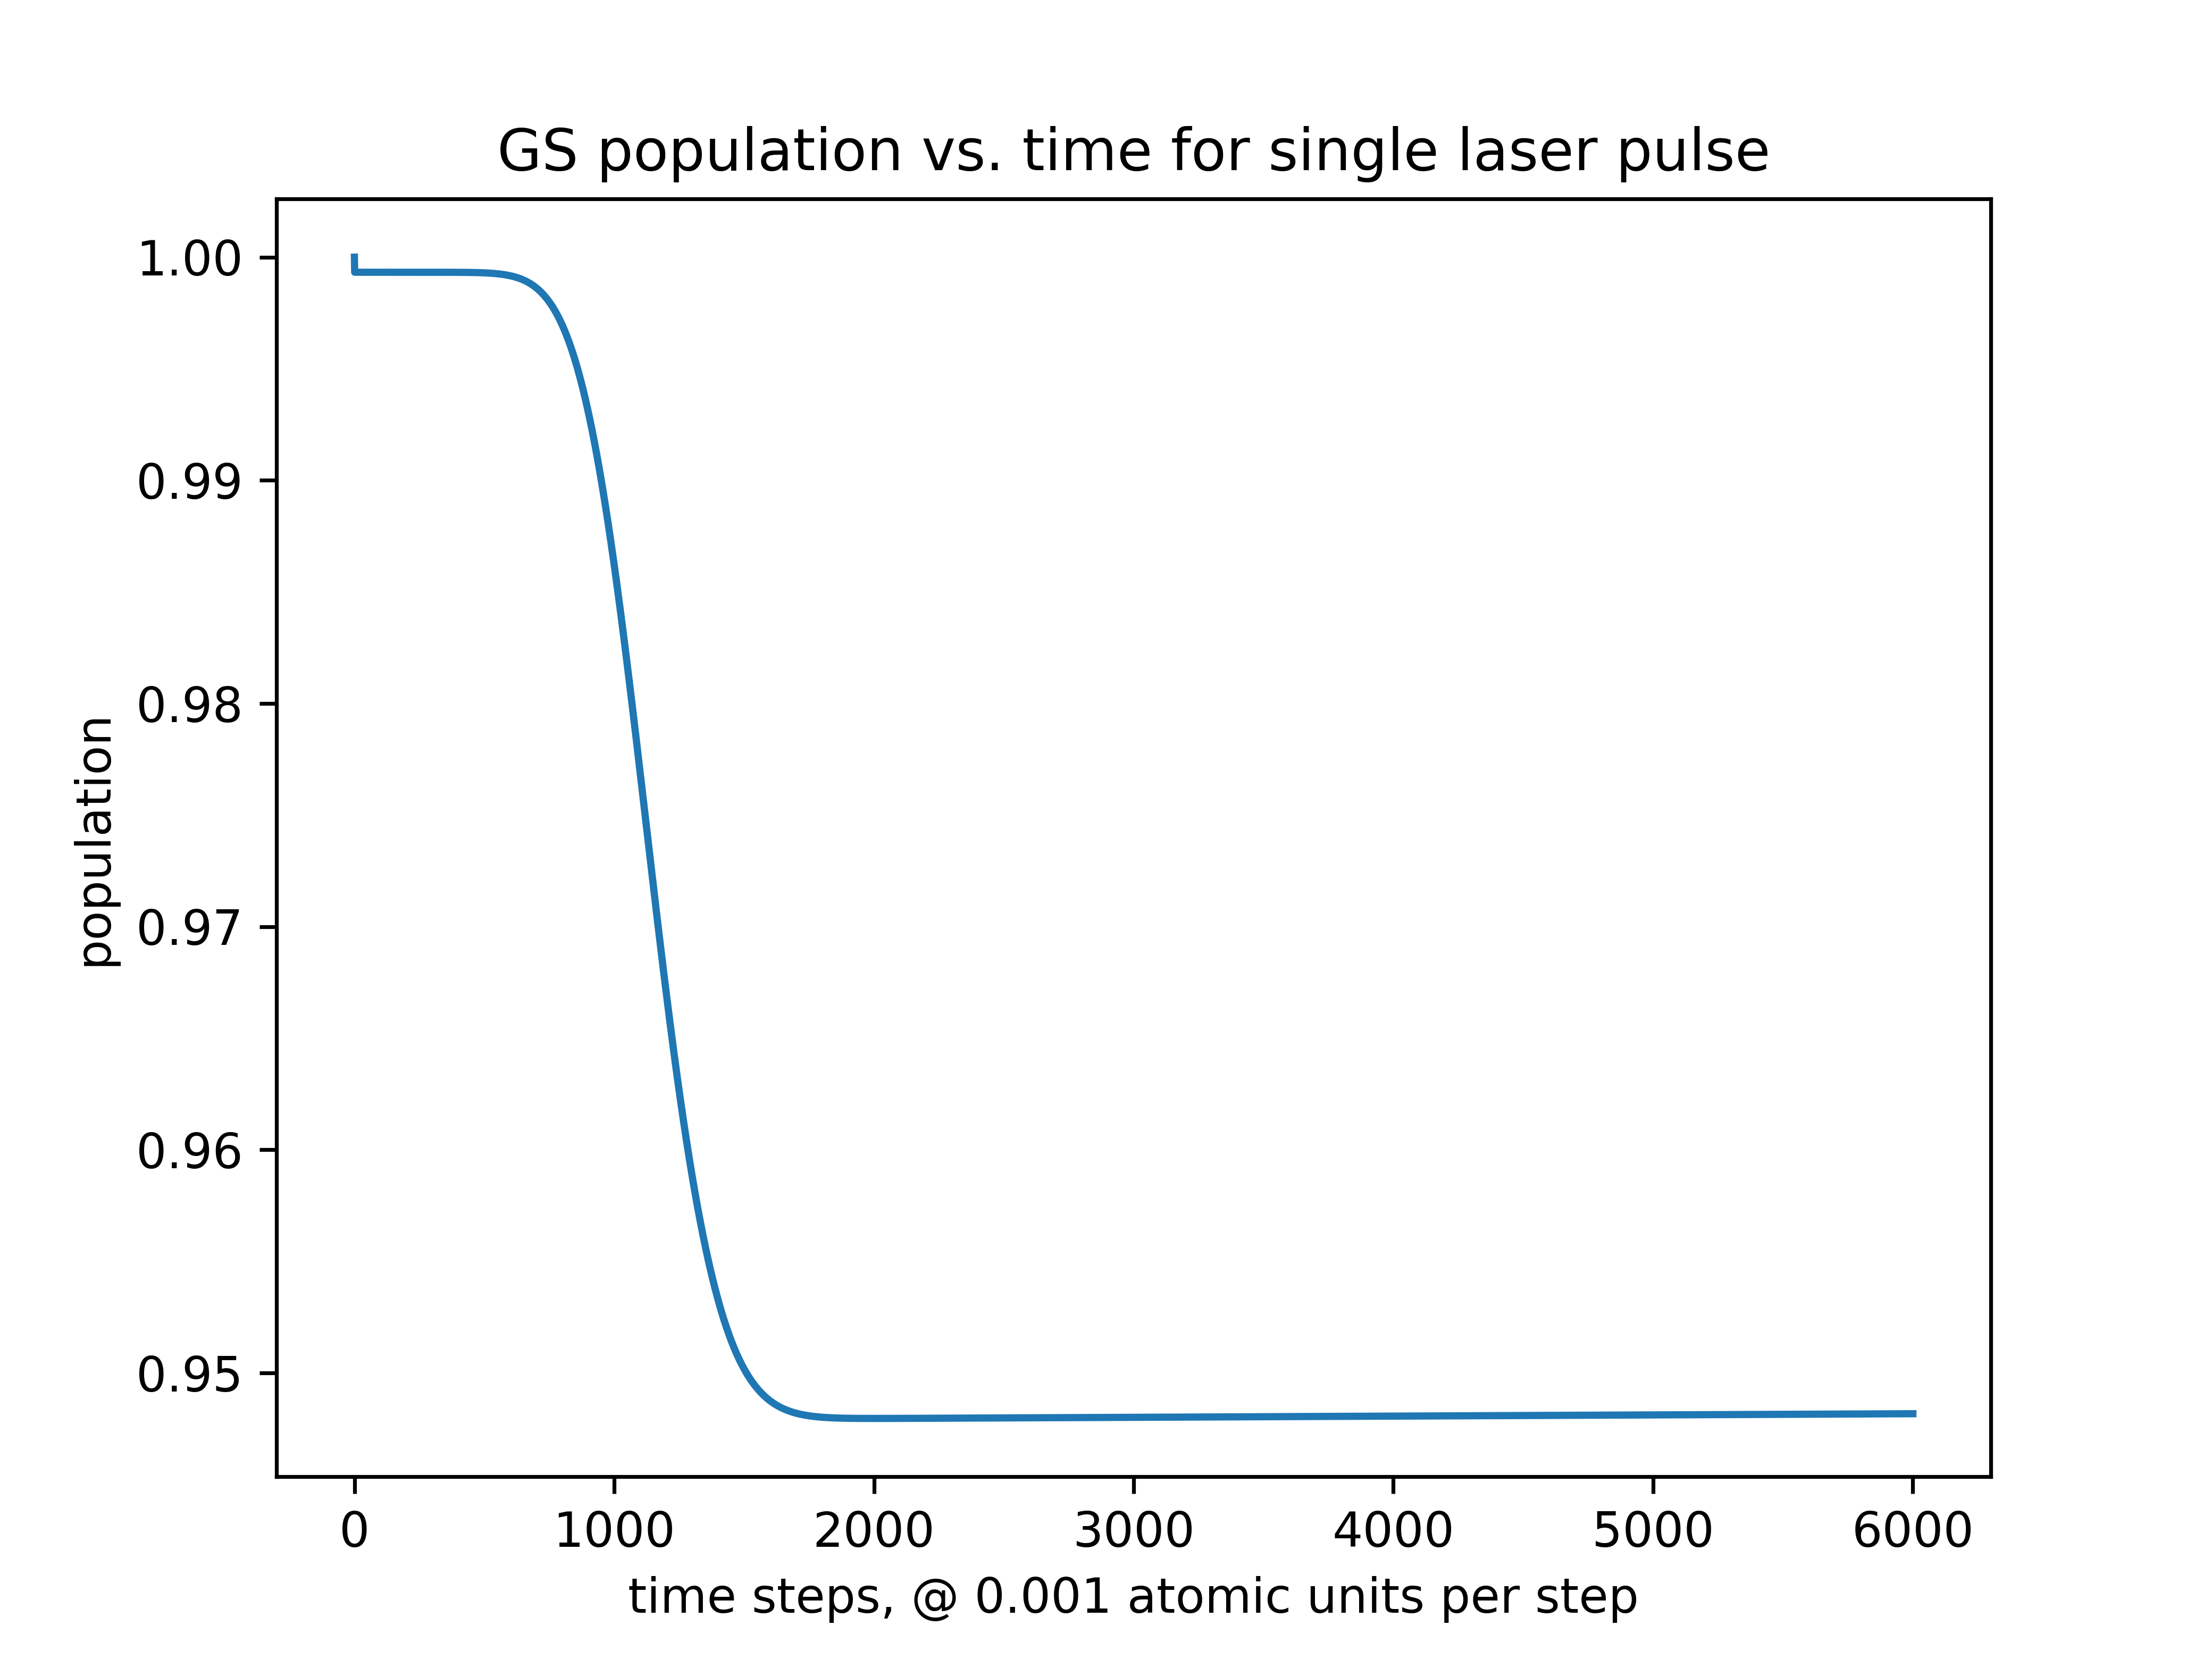
\includegraphics[width=\textwidth]{./GSpopsinglelaser.png}
          \centering
          \caption{Effect of Single Laser Pulse on GS population}
\end{figure}

This graph shows that between around 0.5 and 1.5 atomic units of time into the simulation, the wavefunction is rapidly excited; losing 5\% of the population by 1.5 atomic units of time. Adter this initial loss, the population stays steadily at around 95\% for the rest of the simulation, indicating no further change to its energy.

\section{Multiple Laser Pulses}

We investigate the effects on our system of subjecting it to repeated laser pulses. 

\subsection{Potential Description}
The external potential used in this simulation is similar to the one used in the previous simulation, but with three added to the softcore potential to form the total potential term rather than one. Additionally, two of the simulated pulses have the centres of their gaussian packets shifted to occur at 3 and 5 atomic units of time.

\subsection{Effect On State Evolution}
The graphs in the figure below describe the evolution of the system as it absorbs energy from repeated laser pulses. This differs from the previous investigation of a single laser pulse in that the end result is a system with noticeably higher contributions from excited states than previously, indicating that the system has absorbed more energy. Additionally, the wavefunction of the system at the end shows higher exctited state contributions than in the middle of the simulation - indicating that energy is absorbed both before and after the middle point of the simulation, matching expectations as the laser pulses were staggered to be centred around $\frac{1}{6}, \frac{3}{6}, \text{ and }\frac{5}{6}$ of the simulation.
\begin{figure}[H]
          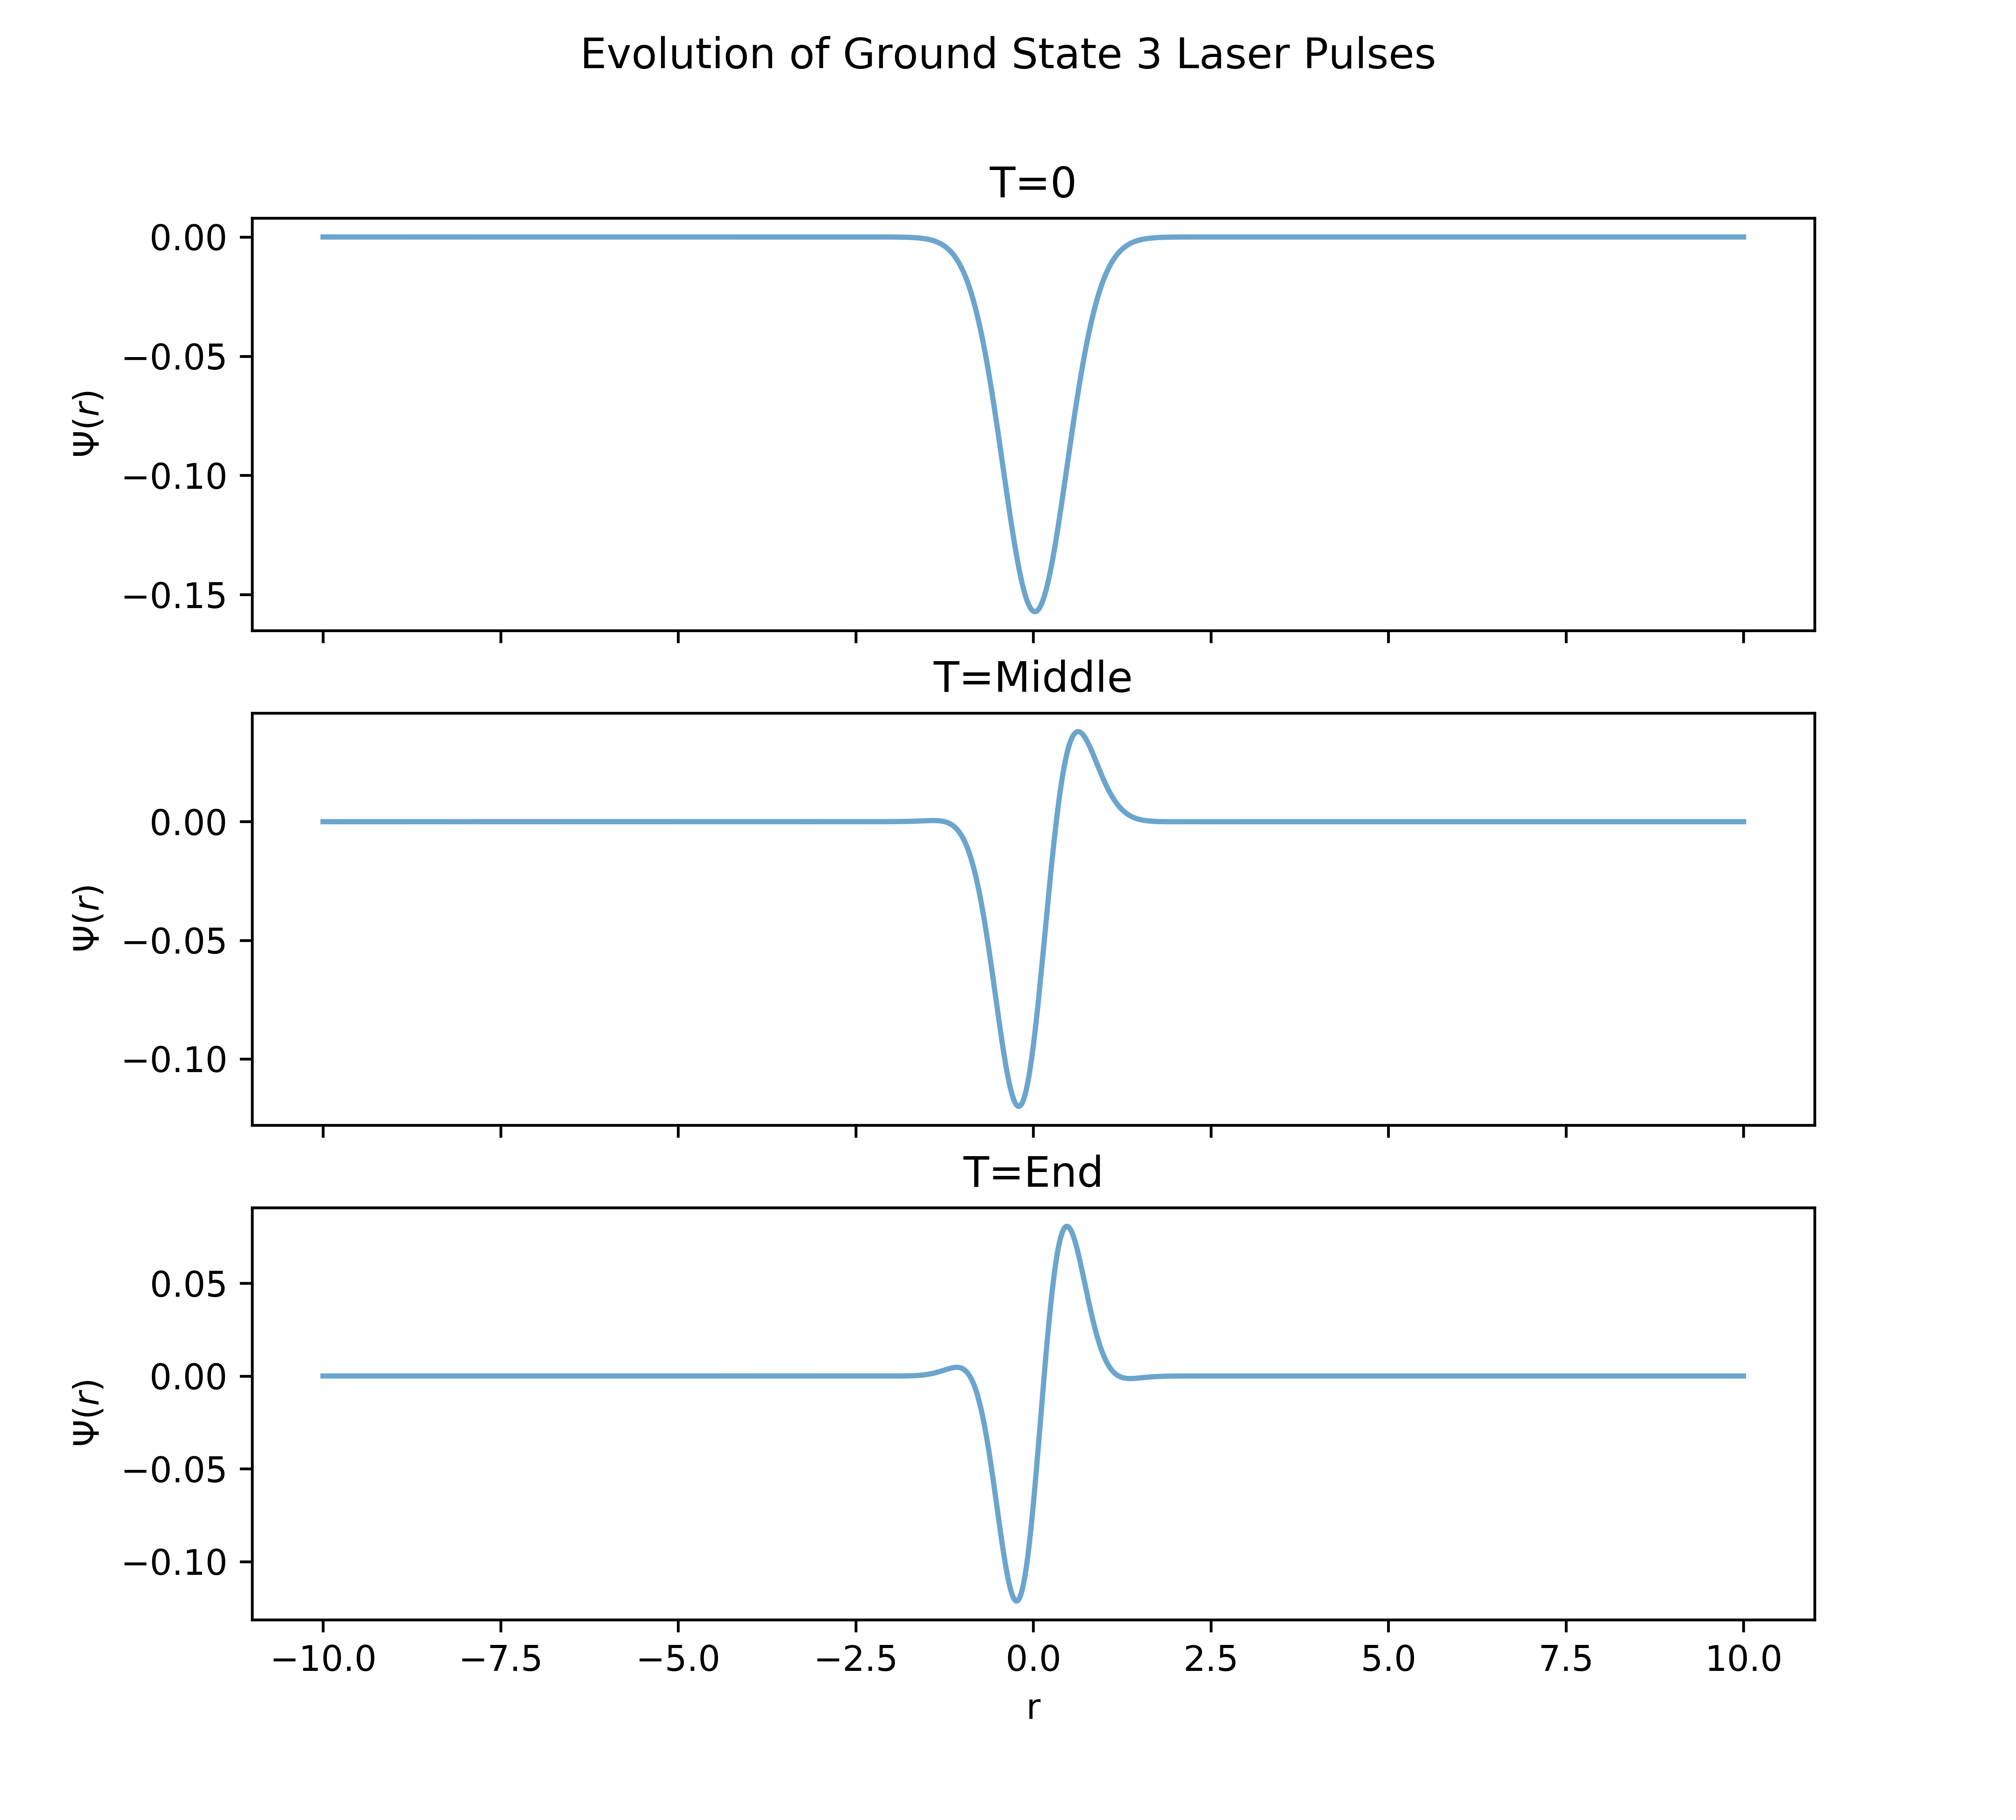
\includegraphics[width=\textwidth]{./GS3LPwavefunction3times.png}
          \centering
          \caption{Effect of Single Laser Pulse on wavefunction}
\end{figure}

The Ground State population was also investigated, with the results shown in Figure 4.6 below, and we can see that there are three distinct drops in population - centred around 1, 3, and 5 atomic units of time; matching when we placed the maxima of the laser pulses. Additionally, we can see that the repeated laser pulses led to a higher overall drop in Ground State population by the end of the simulation, matching the analysis of the evolution of the wavefunction where we noticed higher contributions from excited states than with the single laser pulse.
\begin{figure}[H]
          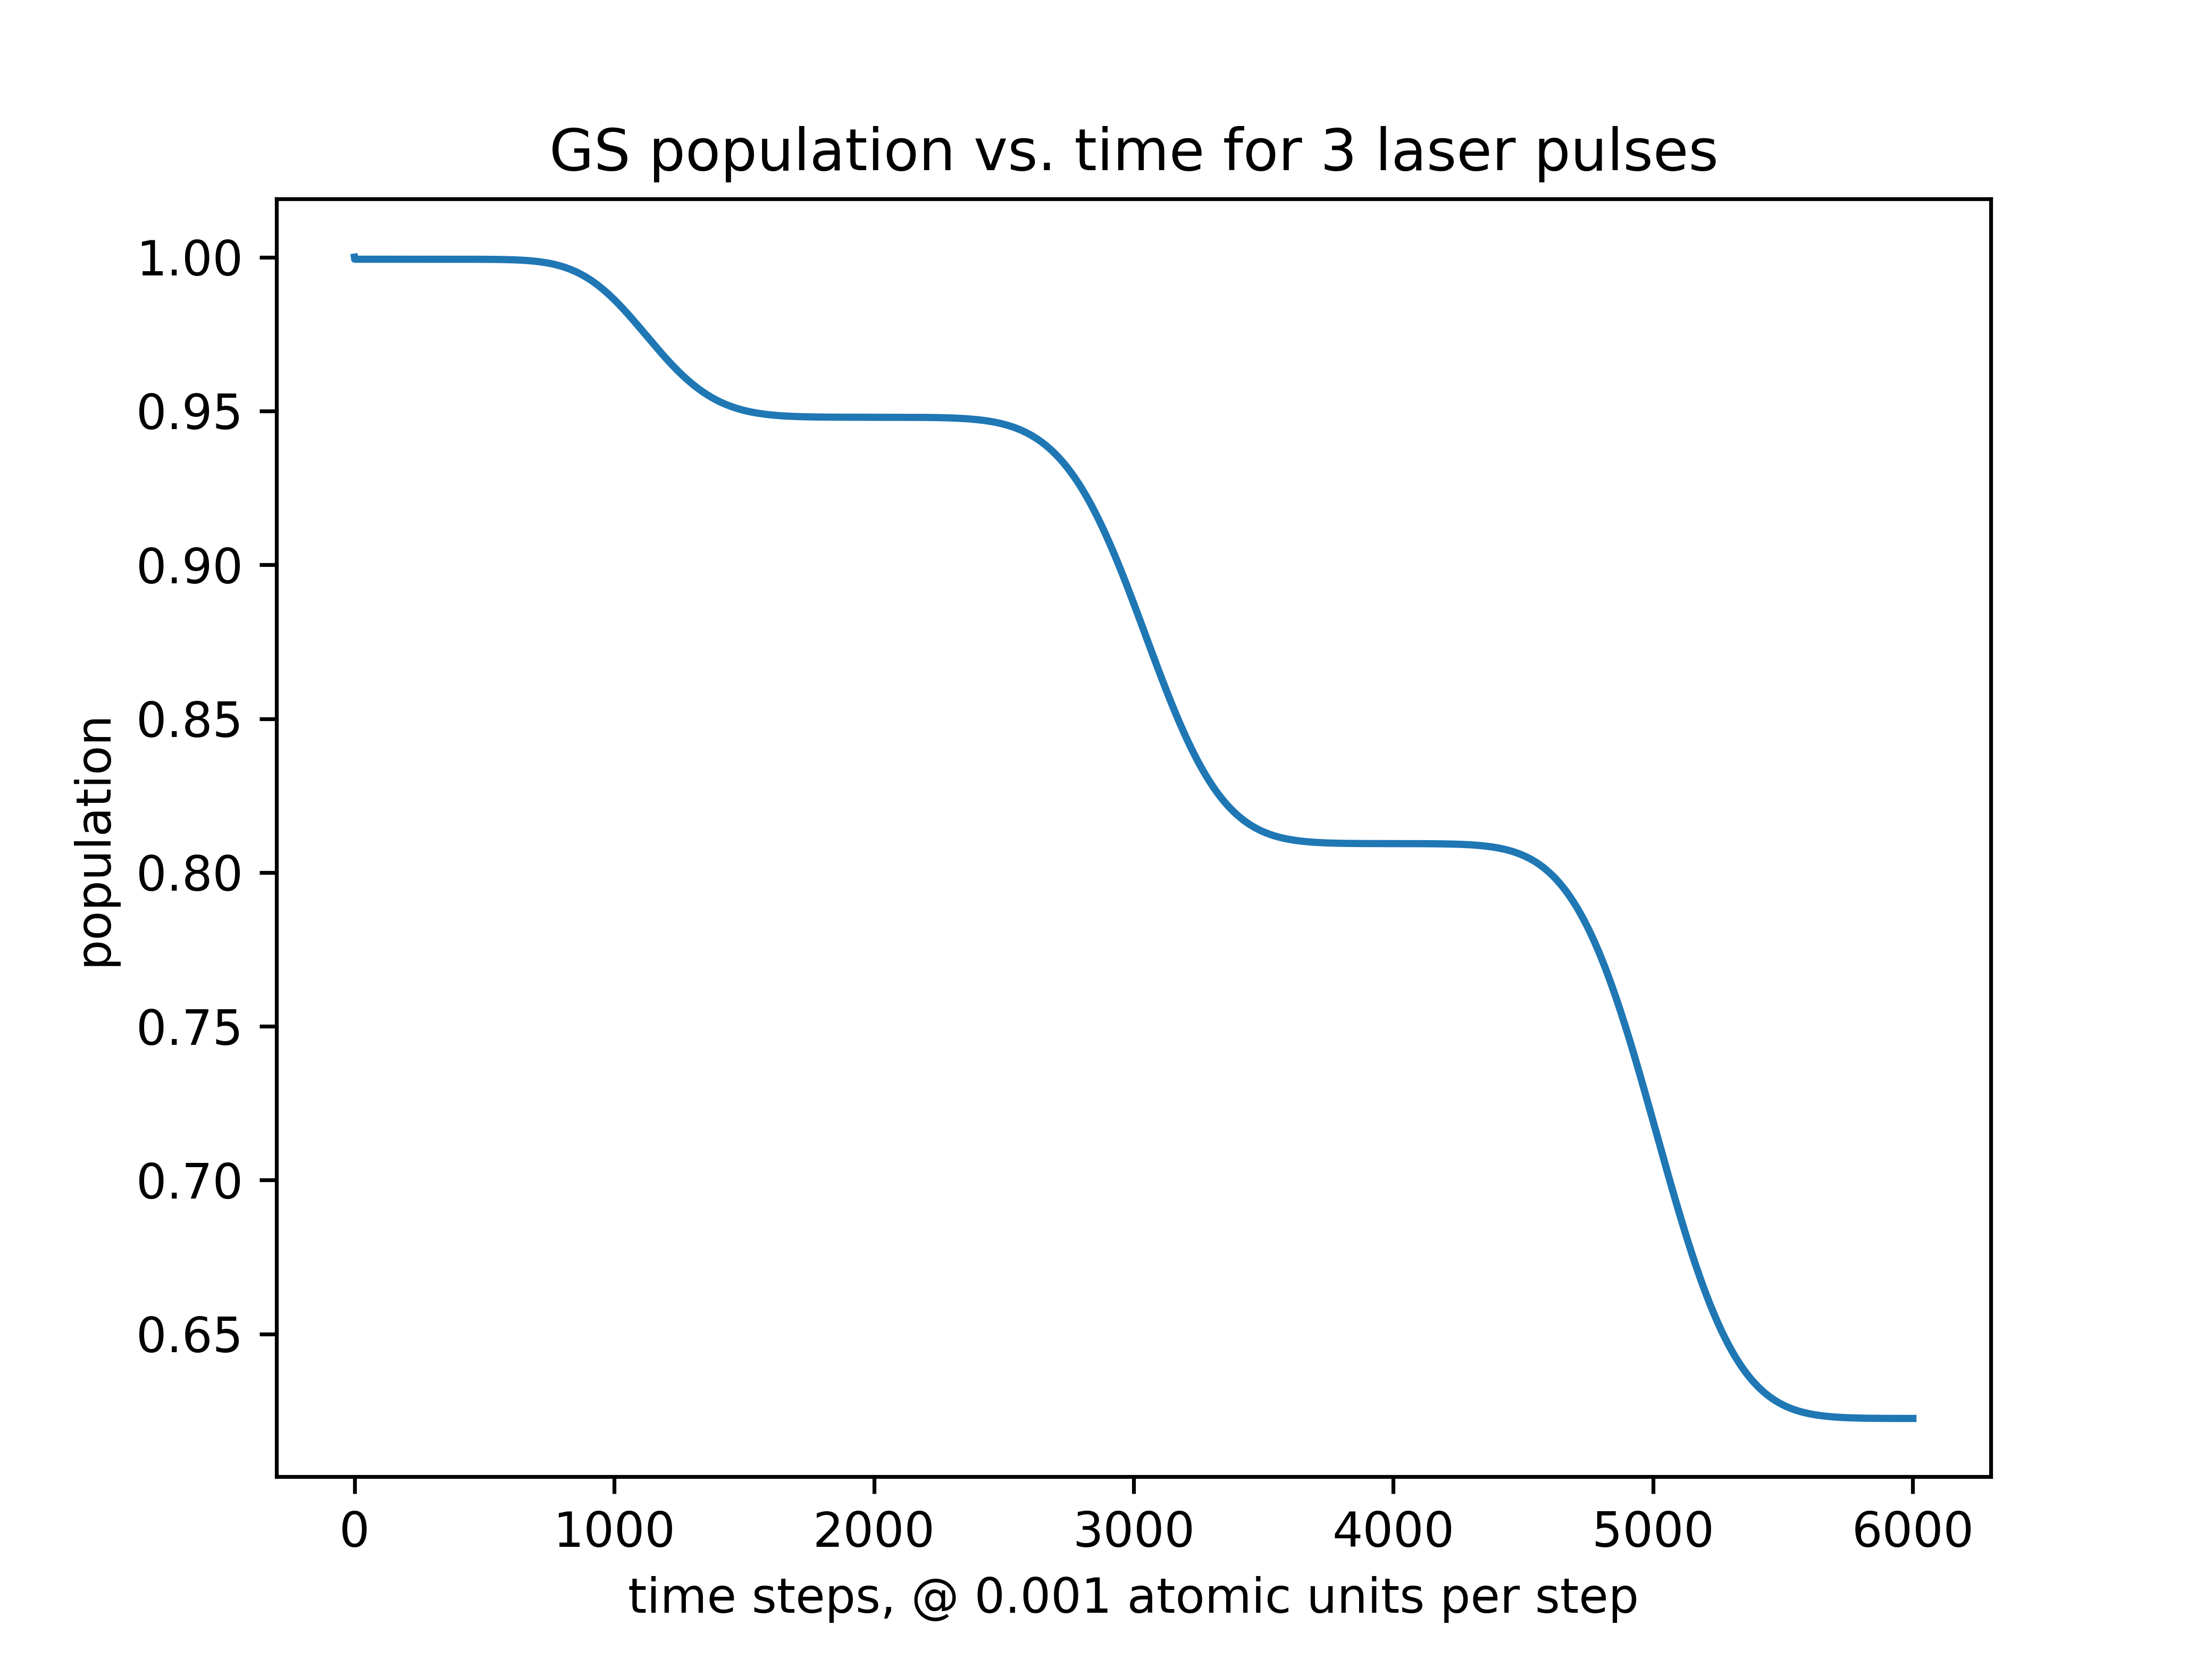
\includegraphics[width=\textwidth]{./GSpop3pulses.png}
          \centering
          \caption{Effect of Single Laser Pulse on GS population}
\end{figure}

\section{Absorbing and Emitting a Photon}
We now look at modelling the situation where our quantum system absorbs some amount of energy (for example from an incoming photon), exciting it to a higher excited state, then releasing an equal amount of energy - i.e. emitting a photon of the same energy and returning to the Ground State.

\subsection{Potential Description}
For this simulation we model the incoming photon in the same way we previously modelled an incoming laser pulse, and then model the emission of the photon in the same way but with an opposite sign. We stagger the point in time that defines the centre of the emission pulse to ensure that the energy from the photon is fully absorbed before being emitted. 

\subsection{Effect On State Evolution}
We can expect the state at the end to match the result of field-free evolution of the initial, ground, state as the energy of the system should have no overall change. Figure 4.7 seems to match this expectation, with the final state showing only one turning point and having a similar shape to the initial state. Additionally, the mid-simulation wavefunction qualitatively seems to have contributions from higher excited states; shown through having an increased number of turning points. This matches our physical expectations, of an initially minimum-energy system being excited and then releasing energy to return to its minimum-energy state.

\begin{figure}[H]
          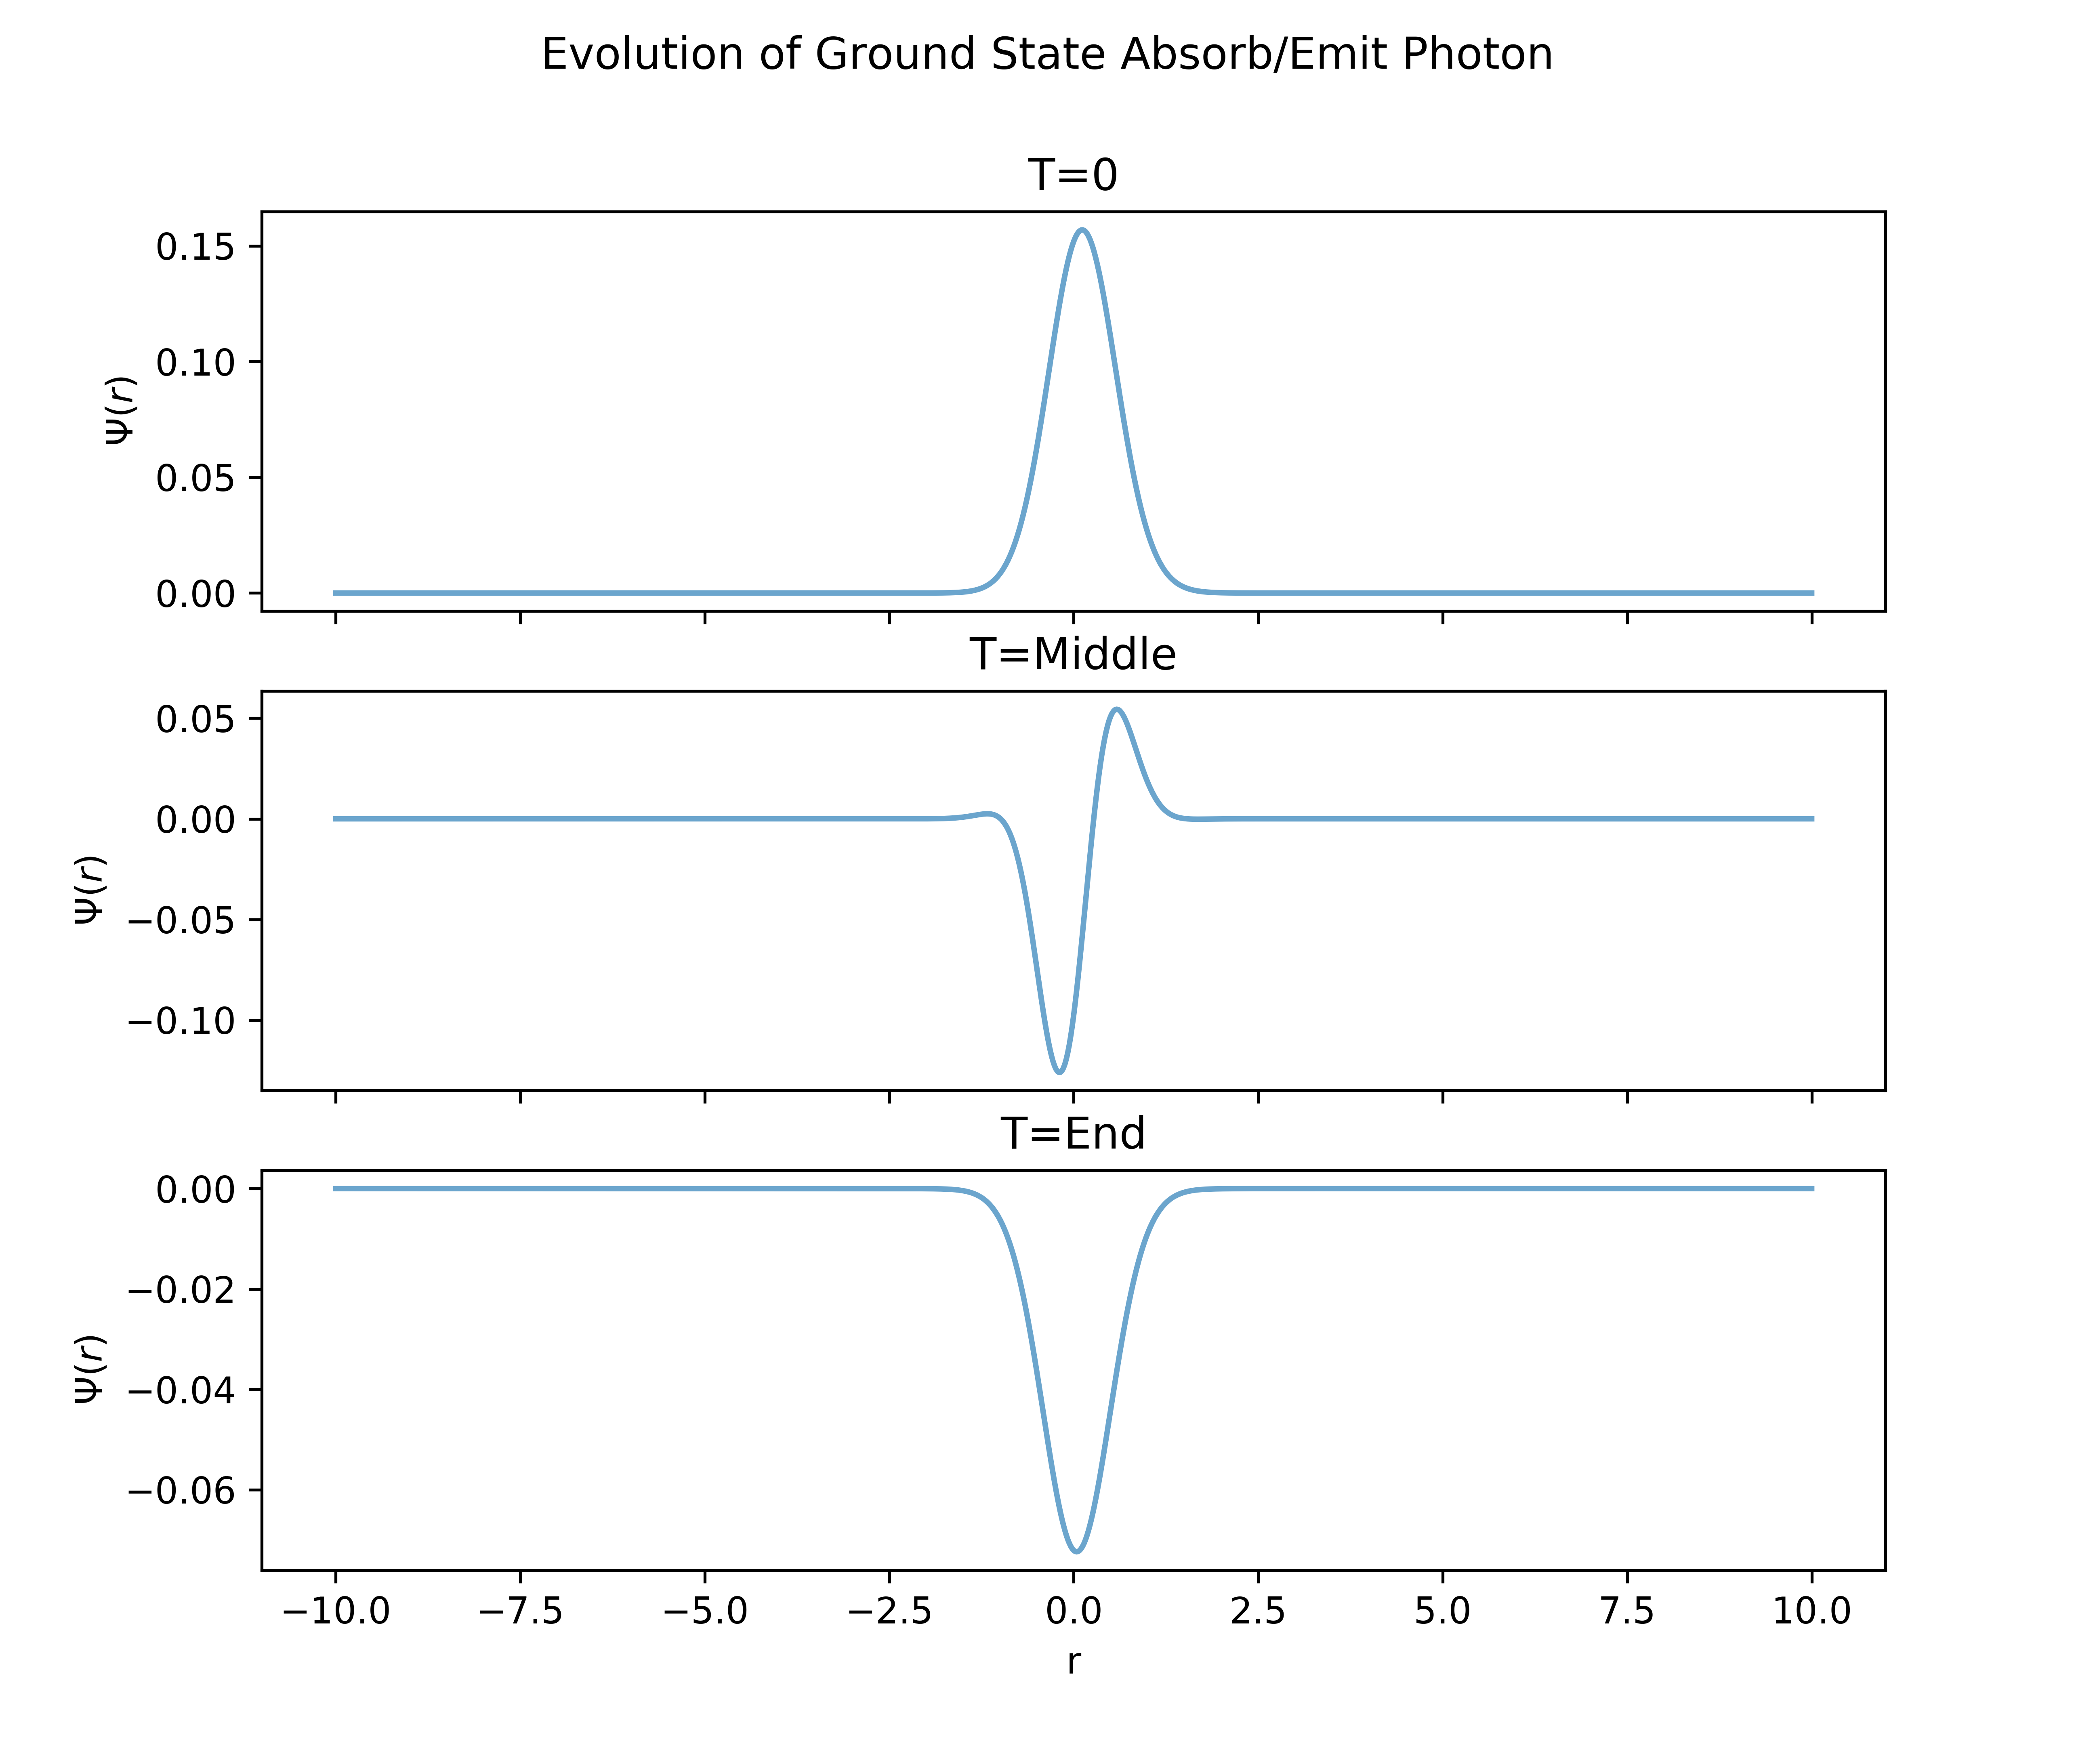
\includegraphics[width=\textwidth]{./GSabsorbemit.png}
          \centering
          \caption{Evolution of System on Absorbing and Emitting a Photon}
\end{figure}

Looking at the change in Ground State population for this simulation, we see that it matches our physical interpretation; the population falls rapidly when absorbing the photon, then is regained when the energy is emitted. 

\begin{figure}[H]
          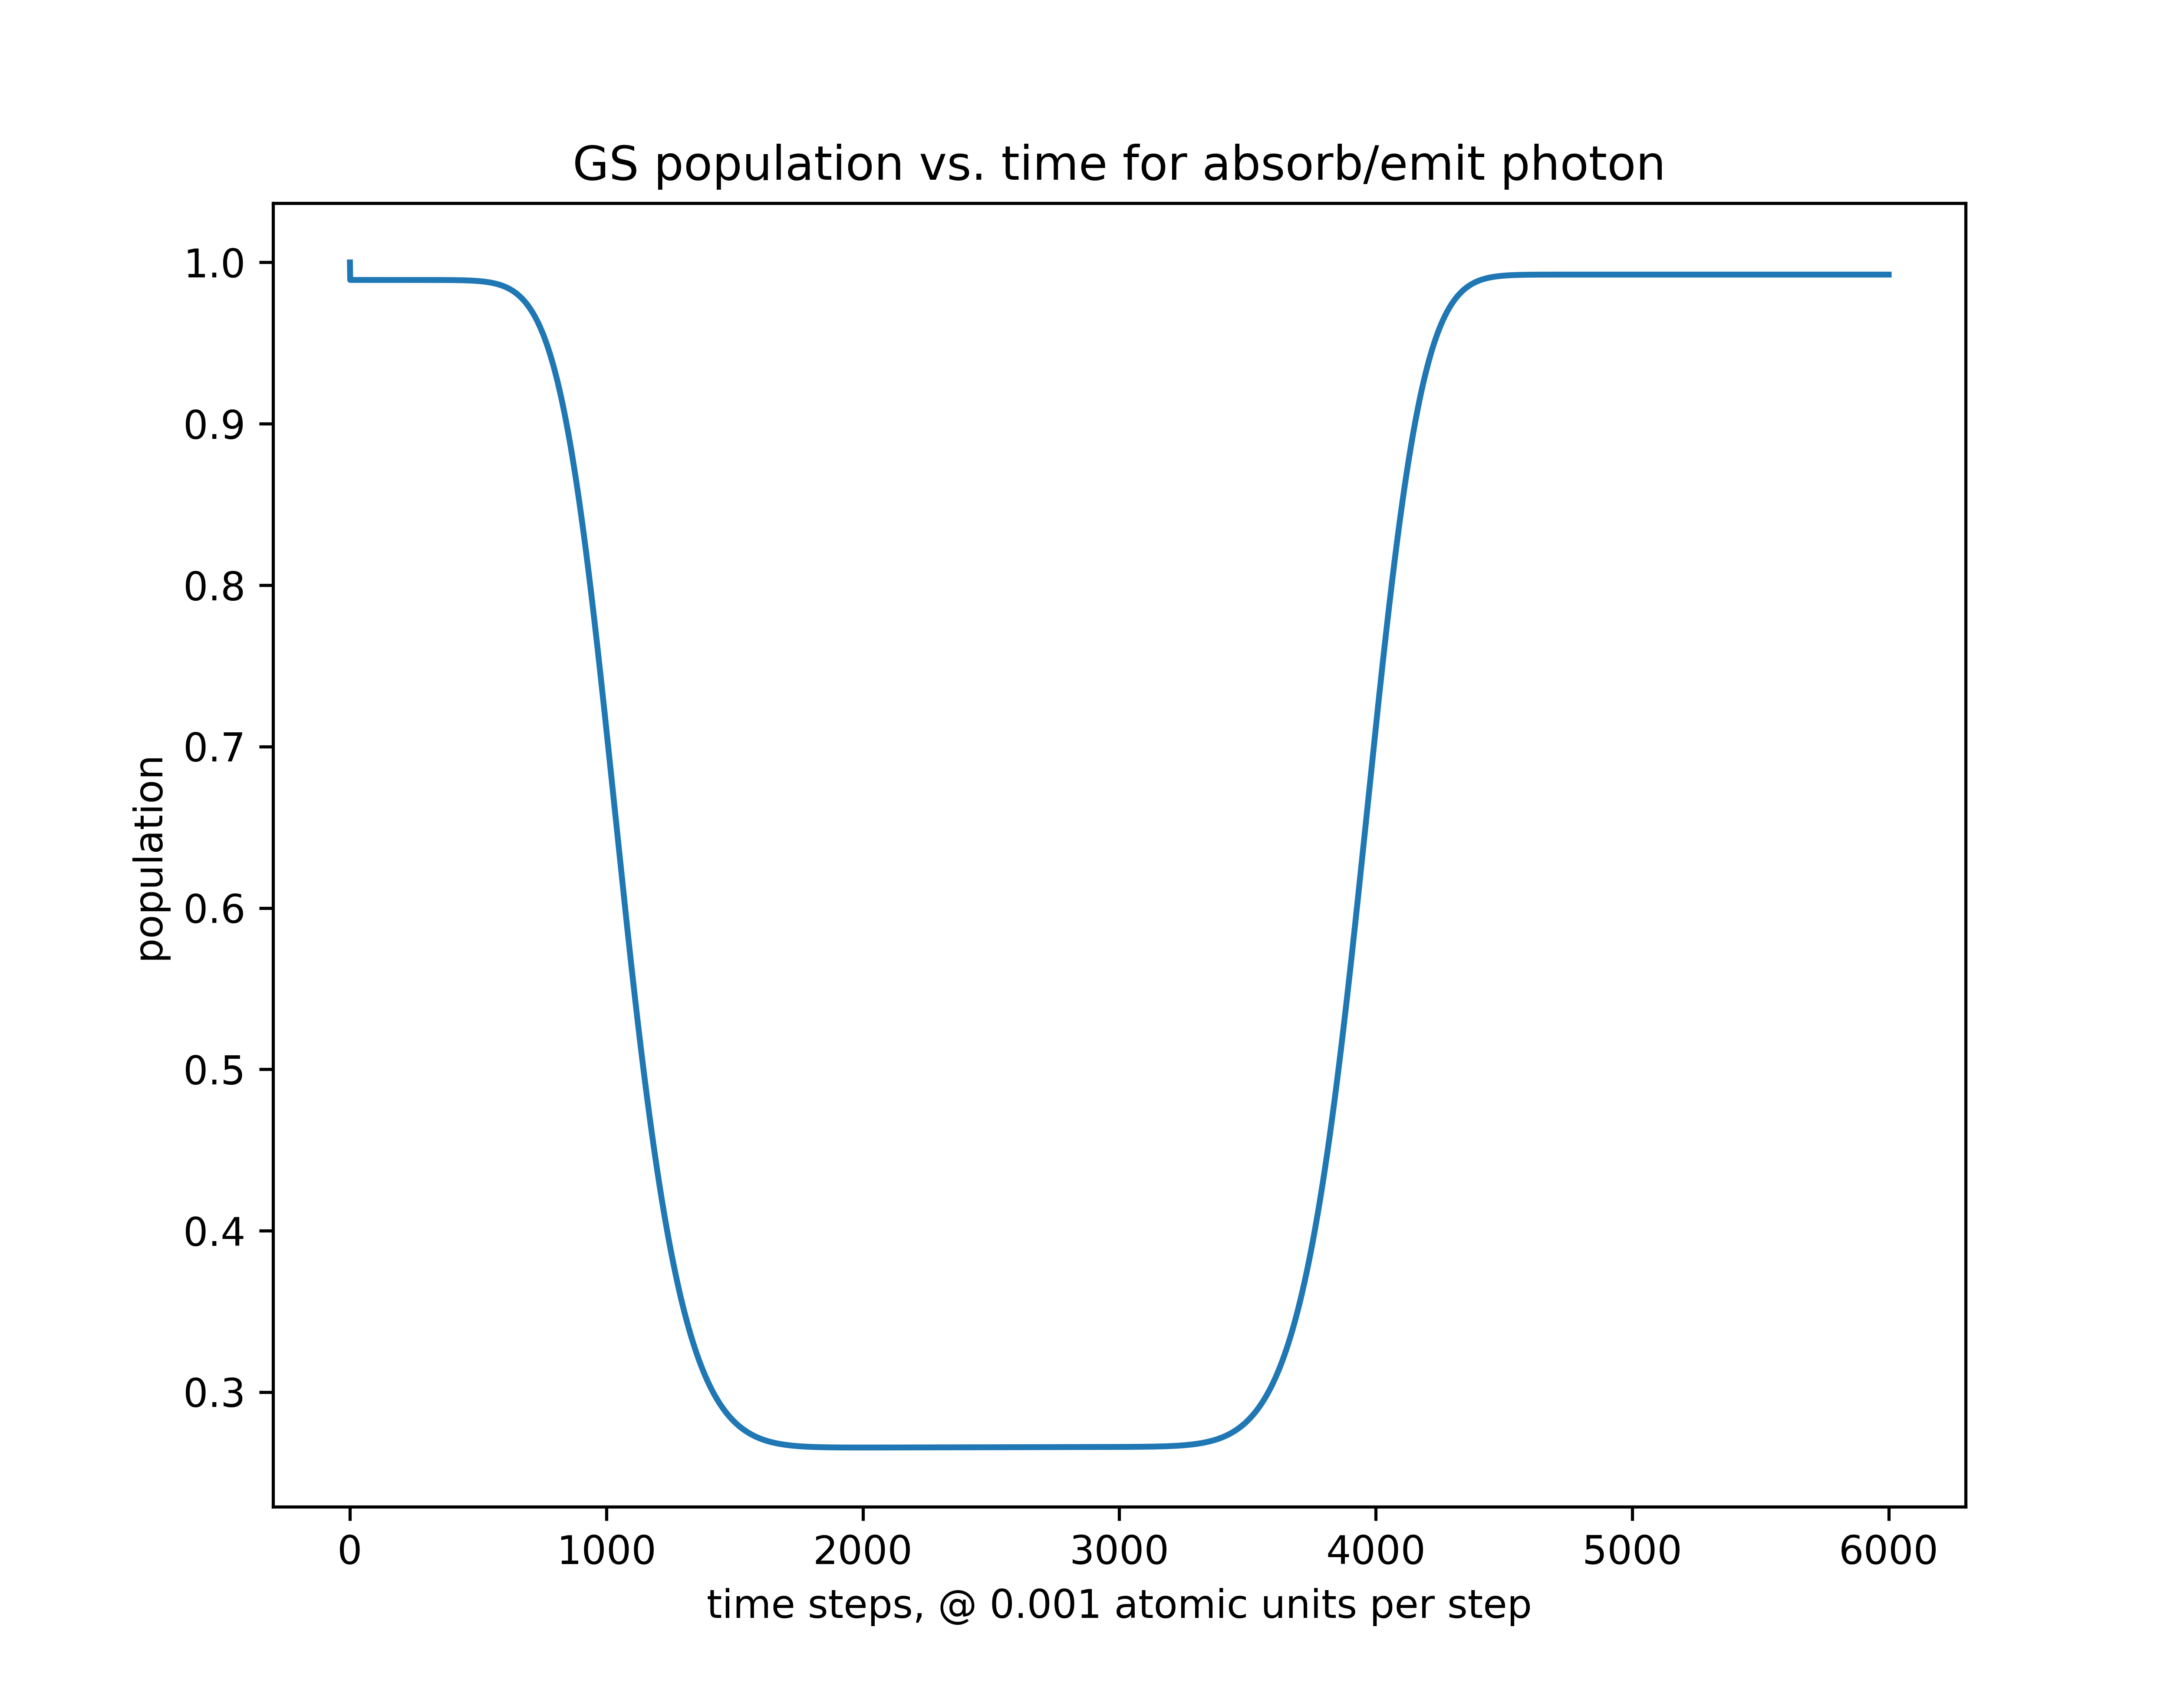
\includegraphics[width=\textwidth]{./GSpopabsorbemitphoton.png}
          \centering
          \caption{Effect of Absorbing and Emitting a Photon on GS Population}
\end{figure}

%----------------------------------------------------------------------------------------
